Um den persönlichen Stundenplan anzuzeigen, muss im Web-Interface der Punkt \enquote{Stundenplan} gewählt werden. \\
\\
Wenn die Seite aufgerufen wird, wird zunächst der modifizierte Stundenplan der aktuellen Woche angezeigt.\\

\begin{figure}[H]
\centering
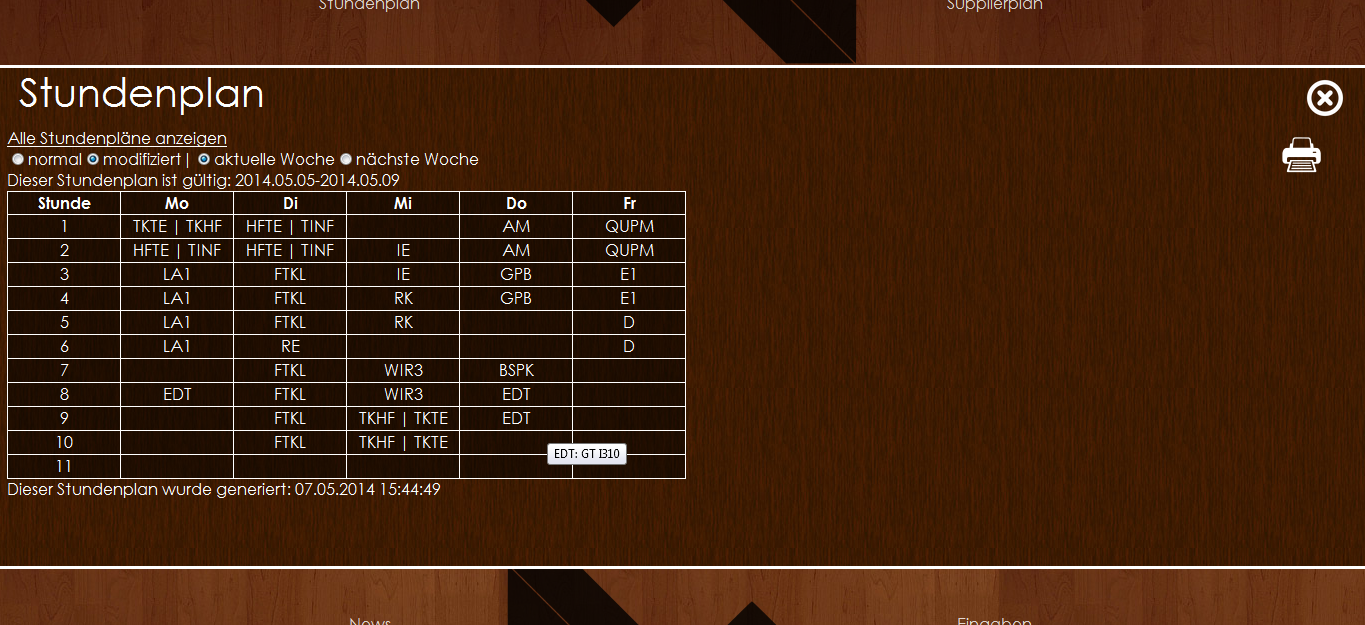
\includegraphics[keepaspectratio=true, width=14cm]{images/screenshots/timetable_mod.png}
\caption{modifizierter Stundenplan mit Popup}
\label{fig:Web_mod_timetable}
\end{figure}

Mittels der Optionen oberhalb der Stundenplanausgabe kann auf den nicht modifizierten Stundenplan umgeschalten werden. Ebenso ist es möglich den modifizierten Stundenplan der nächsten Woche anzeigen zu lassen.
Um das Popup mit den weiteren Informationen anzuzeigen, muss die Maus auf einem der Einträge platziert werden.
\subsection{modifizierter Stundenplan}
Innerhalb des modifizierten Stundenplans werden die Supplierungen der gewählten Woche angezeigt.\\
Wenn bei einer Stunde nur der Lehrer oder der Raum geändert wurde, wird im Popup der betroffene Eintrag verändert. Wenn jedoch in dieser Stunde ein anderes Fach unterrichtet wird, wird im Popup der alte Eintrag durch ein \enquote{-} ersetzt und eine zusätzliche Zeile mit dem neuen Unterrichtsgegenstand, Lehrer und Raum angezeigt.
\subsection{Stundenplan ausdrucken}
Um den eigenen Stundenplan auszudrucken, muss nur im rechten oberen Eck der Druck-Button angeklickt werden.\\
Für einen Administrator ist es zudem möglich alle anderen Stundenpläne auszudrucken. Dazu muss nur auf der Seite \enquote{Alle Stundenpläne} der Druck-Button angeklickt werden, wodurch ein PDF mit dem gerade angezeigten Stundenplan generiert wird.
\subsection{Alle Stundenpläne}
Diese Option ist nur für das Lehrpersonal und die Administration zugänglich.\\\\
Das Lehrpersonal kann nur die Stundenpläne von Klassen einsehen.\\
Beim Öffnen der Seite wird Auswahl zwischen \enquote{Lehrer} und \enquote{Klasse} und eine Eingabezeile angezeigt.\\
\\
Wenn die Option Lehrer gewählt wurde, muss in dieser Zeile das Lehrerkürzel eingegeben werden, bei der Auswahl von Klasse der Klassenname.

\begin{figure}[H]
\centering
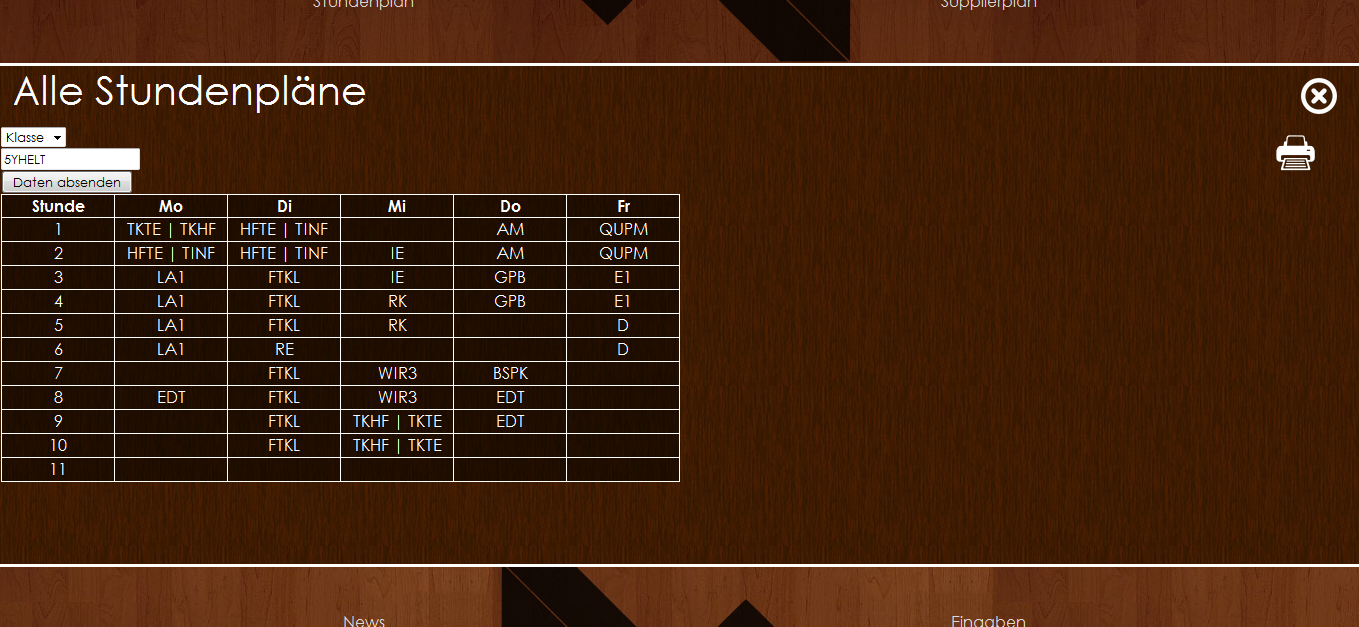
\includegraphics[keepaspectratio=true, width=14cm]{images/screenshots/timetable_all.png}
\caption{Alle Stundenpläne}
\label{fig:Web_all_timetable}
\end{figure}
